%%%%%%%%%%%%%%%%%%%%%%%%%%%%%%%%%%%%%%%%%
% Beamer Presentation
% LaTeX Template
% Version 1.0 (10/11/12)
%
% This template has been downloaded from:
% http://www.LaTeXTemplates.com
%
% License:
% CC BY-NC-SA 3.0 (http://creativecommons.org/licenses/by-nc-sa/3.0/)
%
%%%%%%%%%%%%%%%%%%%%%%%%%%%%%%%%%%%%%%%%%

%----------------------------------------------------------------------------------------
%	PACKAGES AND THEMES
%----------------------------------------------------------------------------------------

\documentclass{beamer}

\mode<presentation> {

% The Beamer class comes with a number of default slide themes
% which change the colors and layouts of slides. Below this is a list
% of all the themes, uncomment each in turn to see what they look like.

%\usetheme{default}
% \usetheme{AnnArbor}
%\usetheme{Antibes}
%\usetheme{Bergen}
%\usetheme{Berkeley}
%\usetheme{Berlin}
%\usetheme{Boadilla}
%\usetheme{CambridgeUS}
%\usetheme{Copenhagen}
%\usetheme{Darmstadt}
\usetheme{Dresden}
%\usetheme{Frankfurt}
%\usetheme{Goettingen}
%\usetheme{Hannover}
%\usetheme{Ilmenau}
%\usetheme{JuanLesPins}
%\usetheme{Luebeck}
%\usetheme{Madrid}
%\usetheme{Malmoe}
%\usetheme{Marburg}
%\usetheme{Montpellier}
%\usetheme{PaloAlto}
%\usetheme{Pittsburgh}
%\usetheme{Rochester}
%\usetheme{Singapore}
%\usetheme{Szeged}
%\usetheme{Warsaw}

% As well as themes, the Beamer class has a number of color themes
% for any slide theme. Uncomment each of these in turn to see how it
% changes the colors of your current slide theme.

%\usecolortheme{albatross}
%\usecolortheme{beaver}
%\usecolortheme{beetle}
%\usecolortheme{crane}
%\usecolortheme{dolphin}
%\usecolortheme{dove}
%\usecolortheme{fly}
%\usecolortheme{lily}
%\usecolortheme{orchid}
%\usecolortheme{rose}
%\usecolortheme{seagull}
%\usecolortheme{seahorse}
%\usecolortheme{whale}
%\usecolortheme{wolverine}

%\setbeamertemplate{footline} % To remove the footer line in all slides uncomment this line
%\setbeamertemplate{footline}[page number] % To replace the footer line in all slides with a simple slide count uncomment this line

%\setbeamertemplate{navigation symbols}{} % To remove the navigation symbols from the bottom of all slides uncomment this line
}

\usepackage{graphicx} % Allows including images
\usepackage{booktabs} % Allows the use of \toprule, \midrule andxs                      % \bottomrule in tables
\usepackage{float}
\usepackage{caption}
\usepackage{subcaption}
\usepackage{listings} %syntax highlighting?
\usepackage{minted}
%\usepackage{subfigure}

%----------------------------------------------------------------------------------------
\graphicspath{ {./images/} }%	TITLE PAGE
%----------------------------------------------------------------------------------------
% \definecolor{mygreen}{cmyk}{0.82,0.11,1,0.25}
% \setbeamertemplate{blocks}[rounded][shadow=false]
% \addtobeamertemplate{block begin}{\pgfsetfillopacity{0.8}}{\pgfsetfillopacity{1}}
% \setbeamercolor{structure}{fg=mygreen}
\setbeamercolor*{block title example}{fg=black,
bg= gray!30}
\setbeamercolor*{block body example}{fg= black,
bg= gray!15}
\graphicspath{ {./images/}{./}{./timgs/} }

\title[How do I SimpleCV?]{A Crash Course on SimpleCV} % The short title appears at the bottom of every slide, the full title is only on the title page

\author{Katherine Scott} % Your name
%\author{Anthony Oliver} % Your name

\institute[SightMachine] % Your institution as it will appear on the bottom of every slide, may be shorthand to save space
{
SightMachine \\ % Your institution for the title page
\medskip
\textit{kat@sightmachine.com}
\textit{anthony@sightmachine.com} % Your email address
}
\date{\today} % Date, can be changed to a custom date

\begin{document}

\begin{frame}
\titlepage % Print the title page as the first slide
\end{frame}

\begin{frame}
\frametitle{Overview} % Table of contents slide, comment this block out to remove it
\tableofcontents % Throughout your presentation, if you choose to use \section{} and \subsection{} commands, these will automatically be printed on this slide as an overview of your presentation
\end{frame}

%----------------------------------------------------------------------------------------
%	PRESENTATION SLIDES
%----------------------------------------------------------------------------------------
\section{Quick Start!}
 \begin{frame}
   \frametitle{Get Started!}
   There are a lot of dependencies for SimpleCV and it is a bit tough for
   beginners. We've brought disks that are ready to go!
   \begin{itemize}
     \item Windows / Linux
       \begin{itemize}
         \item Boot from USB drive.
         \item Alternatively install VirtualBox and the image. 
         \item \url{https://www.virtualbox.org/}
         \end{itemize}
     \item Macs 
       \begin{itemize}
         \item Newer macs are persnikety about booting from a USB drive.
         \item Install virtual box and the ISO and go to town. 
         \end{itemize}
     \item When you get home install from SuperPack or preferably source libs.
       \begin{itemize}
         \item take awhile and is not a perfect science.
         \item \url{https://github.com/ingenuitas/SimpleCV}
         \item If you want to contribute this is a great place to start.
         \end{itemize}
    \end{itemize}
 \end{frame}

%----------------------------------------------------------------------------------------
\begin{frame}
  \frametitle{About the tutorial}
  \begin{itemize}
    \item It will be a lot of live coding. I'll lead, you follow along.
    \item If you have a question feel free to interrupt. 
    \item If you are having an issue raise a flag. Anthony will help
      you. 
    \end{itemize}
\end{frame}


%------------------------------------------------
\section{What is SimpleCV?} % Sections can be created in order to organize your presentation into discrete blocks, all sections and subsections are automatically printed in the table of contents as an overview of the talk
%------------------------------------------------

\subsection{What makes up SimpleCV?} % A subsection can be created just before a set of slides with a common theme to further break down your presentation into chunks

% ------------------------------------------------
\begin{frame}
\frametitle{What Makes Up SimpleCV?}
\begin{figure}
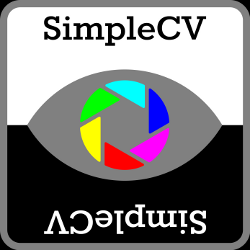
\includegraphics[width=0.5\linewidth]{simplecv.png}
\end{figure}
\end{frame}

% ------------------------------------------------

\begin{frame}
\frametitle{SimpleCV != OpenCV }
\begin{figure}
  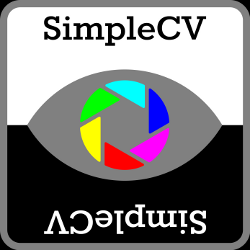
\includegraphics[width=0.2\linewidth]{simplecv.png}
\end{figure}
\begin{itemize}
  \item OpenCV is really busy, we help by wrapping python.
  \item We add lots of other fun stuff (OCR, Barcodes, etc.)
  \item We are not competing, we are complementing. 
  \item Purposes are different. Python is great for prototyping. C++ great for embedded.
\end{itemize}
\end{frame}

% ------------------------------------------------

\begin{frame}
  \frametitle{Core Dependencies}
  \begin{itemize}
  \item \href{http://www.opencv.org}{OpenCV} Python Bindings
  \item \href{http://docs.scipy.org/doc/}{Numpy}
  \item \href{http://docs.scipy.org/doc/}{SciPy}
  \item SciKits Learn and \href{http://orange.biolab.si/}{Orange}
  \item \href{http://www.pygame.org}{PyGame} (this is going away)
  \item \href{http://www.pythonware.com/products/pil/}{Python Imaging Library (PIL)}
  \item \href{http://ipython.org/}{ipython}
  \item PIL (Python Imaging Library)
  \end{itemize}
\end{frame}

% ------------------------------------------------

\begin{frame}
  \frametitle{Optional Dependencies}
  \begin{itemize}
  \item Barcodes- Zebra Crossing \href{https://code.google.com/p/zxing/}{ZXIng}
  \item Optical Character Recognition (OCR) - \href{https://code.google.com/p/tesseract-ocr/}{Tesseract}
  \item Beautiful Soup 
  \item Kinect Support - freenect 
  \item Unit Tests - nose
  \item Web Stuff - flask / CherryPy
  \item Arduino - pyfirmata
  \item Many Many Many more. 
  \end{itemize}
\end{frame}

% ------------------------------------------------

\begin{frame}
  \frametitle{This is why we put everything in a superpack / virtual
    box / bootable drive}
  \begin{itemize}
  \item Just get to the core library functions.
  \item We encourage you to install the full library when you get
    home.
  \item Help is available if you need it. 
  \end{itemize}
\end{frame}

% ------------------------------------------------
\begin{frame}
\frametitle{Getting Help after the tutorial.}
\begin{figure}
  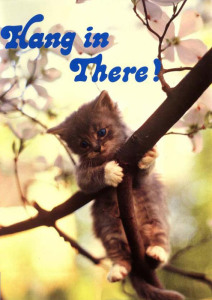
\includegraphics[width=0.2\linewidth]{hang-in-there-cat.jpg}
\end{figure}
\begin{itemize}
  \item Primary Source: \url{http://help.simplecv.org/questions/}
  \item Documentation \url{http://www.simplecv.org/docs/}
  \item Tweet at us: $@$Simple\textunderscore CV
  \item Another Good Resource: \url{http://www.reddit.com/r/ComputerVision}
\end{itemize}
\end{frame}

% ------------------------------------------------
\begin{frame}
\frametitle{On the Printed Page}

 \begin{figure}
%   \begin{subfigure}
     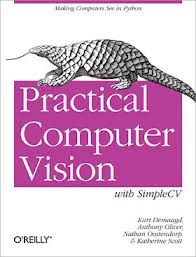
\includegraphics[width=0.4\linewidth]{SimpleCVBook.jpg}
%   \end{subfigure}
%   \begin{sub-figure}
     \quad
     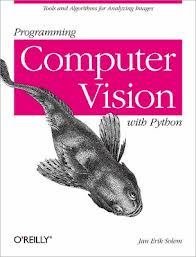
\includegraphics[width=0.4\linewidth]{JanEricBook.jpg}
     \caption{Two books about using Python for Computer Vision}
%   \end{subfigure}
 \end{figure}

\end{frame}

% ------------------------------------------------
\begin{frame}
\frametitle{So why are we doing this?}

\begin{itemize}
  \item We are really nice people who believe in Python and Open
    Source.
  \item We are trying to disrupt industrial quality control systems.
\end{itemize}
\begin{figure}
  
\includegraphics[width=0.6\linewidth]{SightMachineLogo.png}
\end{figure}

\end{frame}

% ------------------------------------------------
\begin{frame}
\frametitle{Early Prototypes}

\begin{figure}
  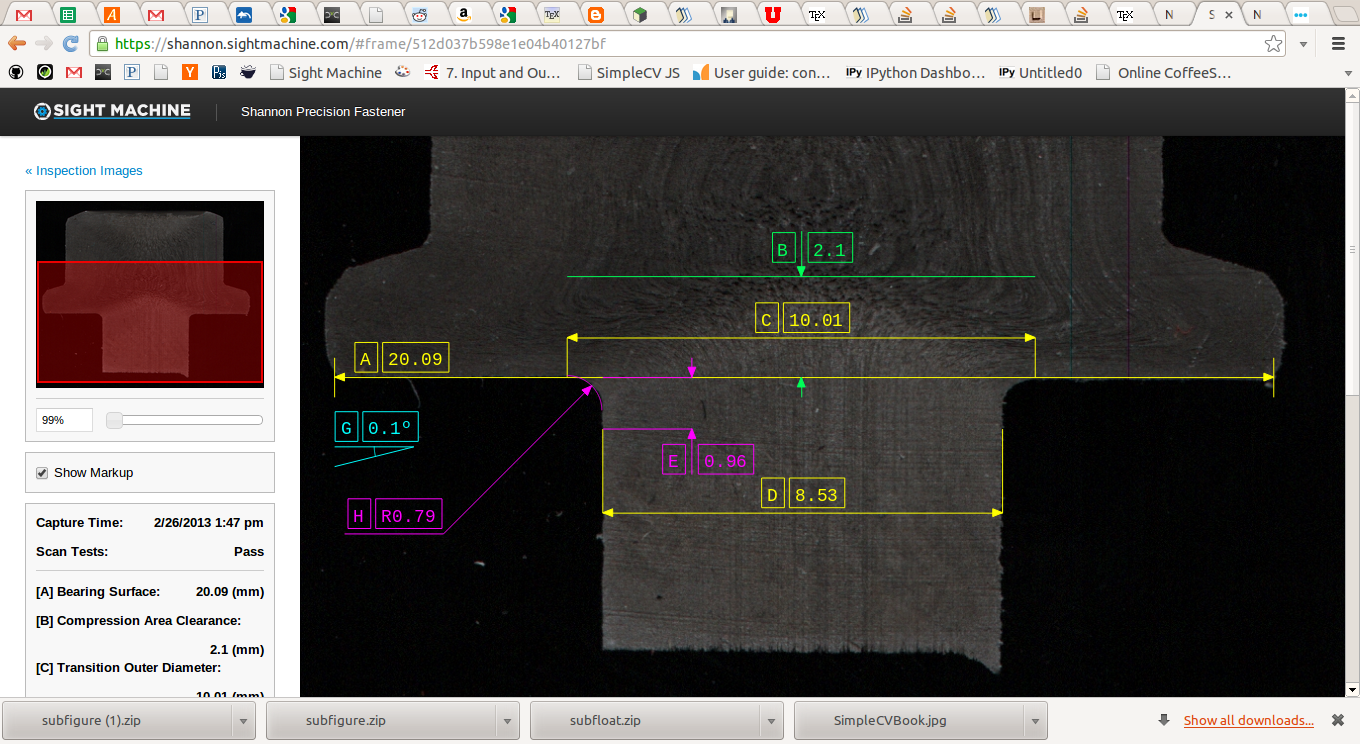
\includegraphics[width=0.9\linewidth]{shannon.png}
  \caption{Early Customer - Industrial Fastener Morphology
      and Metallurgy }
\end{figure}

\end{frame}
% ------------------------------------------------
\begin{frame}
\frametitle{Early Prototypes}

\begin{figure}
  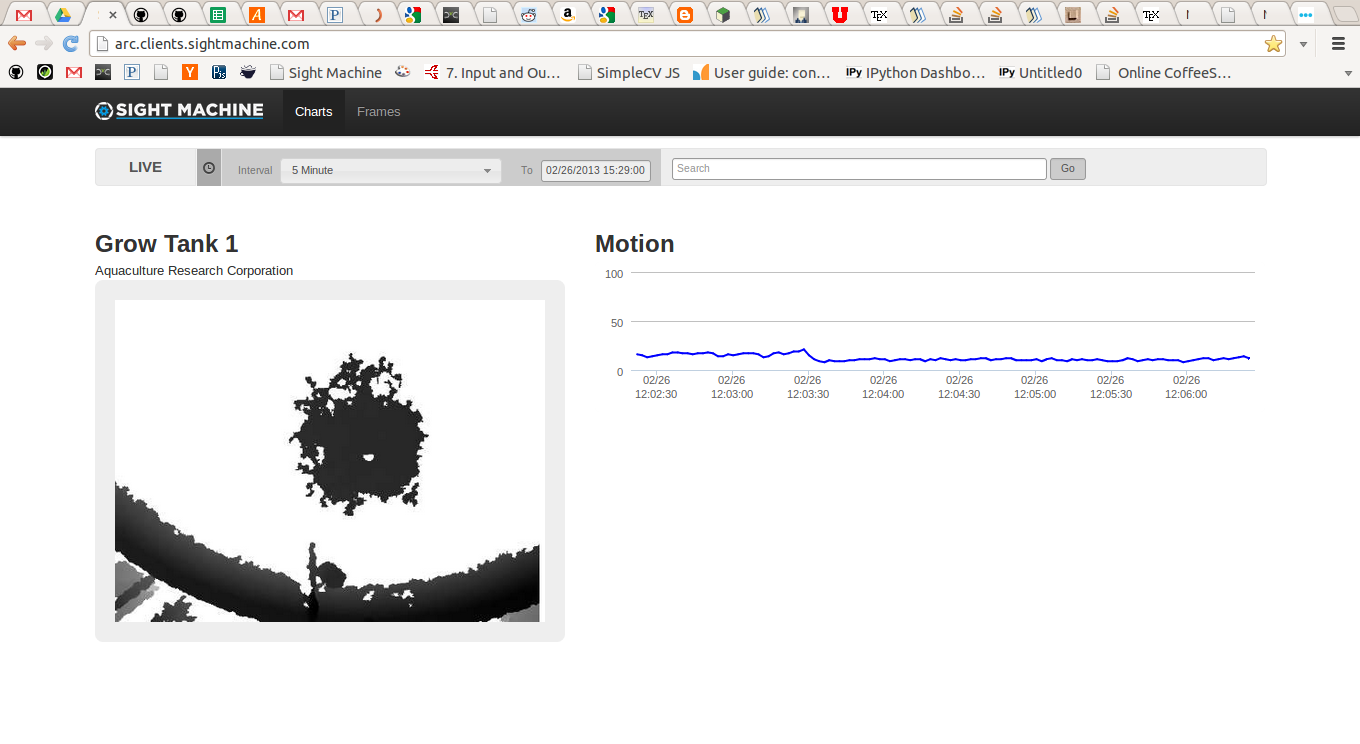
\includegraphics[width=0.9\linewidth]{arc.png}
  \caption{Early Customer - Aquaponics Research Facility}
\end{figure}

\end{frame}

\section{SimpleCV}
\subsection{Getting Started}

% ------------------------------------------------
\begin{frame}
\frametitle{How do I SimpleCV?}

\begin{figure}
  
\includegraphics[width=0.6\linewidth]{howdoi.jpg}
\end{figure}

\end{frame}

 
% ------------------------------------------------
\begin{frame}
\frametitle{Where do I write my code?}

\large{So how do I SimpleCV?}
\begin{itemize}
\item In a python file, just like any other library.
\item In a command line REPL like iPython.
\item In the browser using iPython Notebooks (we'll use this today).
\end{itemize}
We really like iPython. It is kinda like using Matlab without the \$ 5000
per seat license cost. 
\end{frame}

%------------------------------------------------

\begin{frame}
\frametitle{How does fit into a work flow?}
At SightMachine we roughly use these three tools 
for different parts of our workflow.
\begin{table}
\begin{tabular}{l l }
\toprule
\textbf{Tool} & \textbf{Uses} \\
\midrule
iPython REPL & Prototypes, Sanity Checks, Etc \\
iPython Web Notebook & Testing and Development \\
Python Files  & Deployment Code \\
\bottomrule
\end{tabular}
\caption{SimpleCV Workflow}
\end{table}
\end{frame}


% ------------------------------------------------

\begin{frame}[fragile] % Need to use the fragile option when verbatim is used in the slide
\frametitle{SimpleCV Hello World as a Script}
\begin{example}[HelloWorld.py]
 \inputminted[linenos=true, tabsize=4,
 fontsize=\small]{python}{HelloWorld.py}
\end{example}
\end{frame}
% ------------------------------------------------
\begin{frame}
\frametitle{How do I run Hello World?}
\begin{itemize}
\item Run the py file with $python$ $HelloWorld.py$ in the command.
\item Close it by pressing $esc$ or $ctrl-c$
\end{itemize}
\begin{figure}
  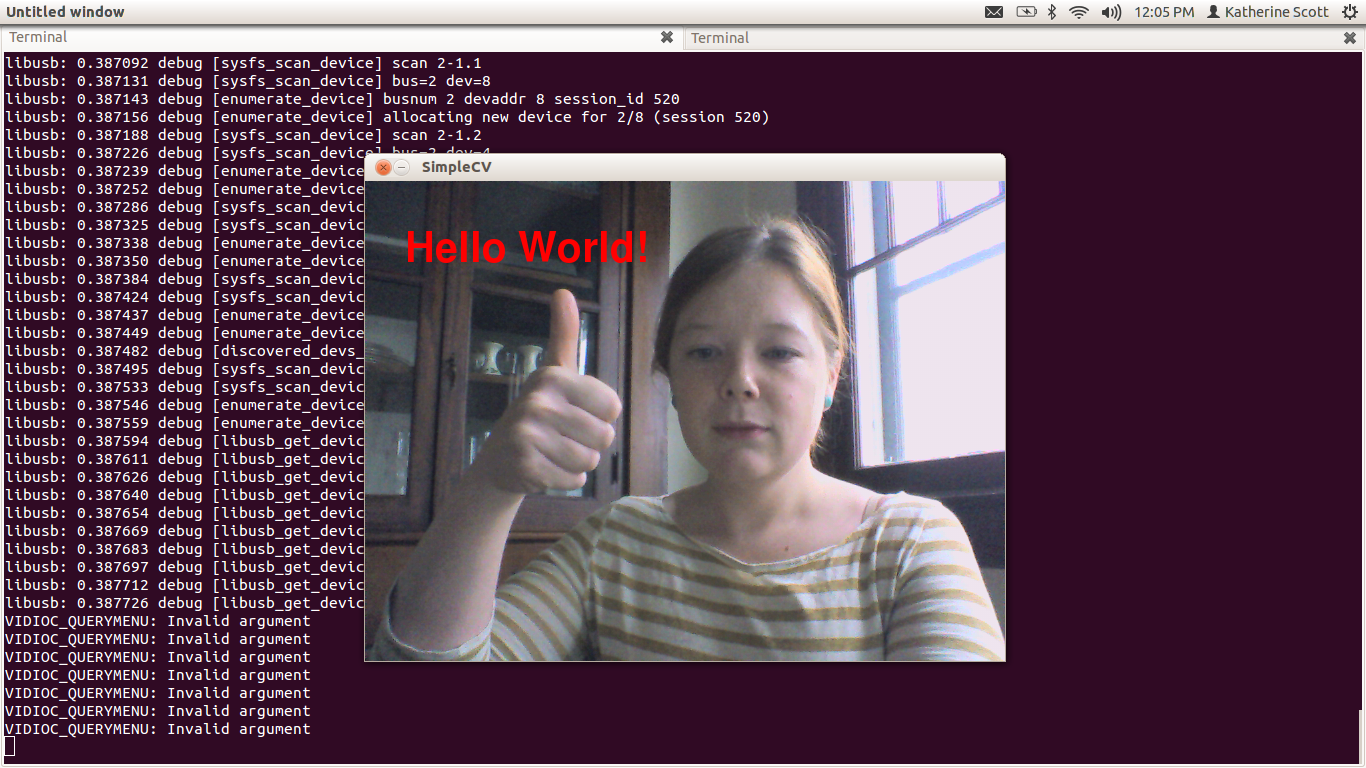
\includegraphics[width=0.9\linewidth]{HelloWorld1.png}
\end{figure}
\end{frame}

% ------------------------------------------------
\begin{frame}
\frametitle{The SimpleCV Shell - Custom iPython REPL}
Sometimes you just want to test an idea without writing a full
script. For this reason we created the SimpleCV shell, which is a
custom ipython instance. The SimpleCV shell will allow you to:
\begin{itemize}
\item Test your ideas in a REPL similar to Matlab.
\item Access the SimpleCV documentation. 
\item Import modules that you are working with to test.
\item Run through an interactive tutorial. 
\end{itemize}
\end{frame}

%------------------------------------------------
\subsection{SimpleCV Shell}
\begin{frame}[fragile] % Need to use the fragile option when verbatim is used in the slide
\frametitle{Starting the SimpleCV Shell}
In OSX and Linux just type $simplecv$ at the command line. On Windows
you just click on the SimpleCV icon. 
\begin{example}[Shell Basics]
\begin{minted}[fontsize=\tiny]{python}
+-----------------------------------------------------------+
 SimpleCV 1.3.0 [interactive shell] - http://simplecv.org
+-----------------------------------------------------------+
Commands: 
	"exit()" or press "Ctrl+ D" to exit the shell
	"clear" to clear the shell screen
	"tutorial" to begin the SimpleCV interactive tutorial
	"example" gives a list of examples you can run
	"forums" will launch a web browser for the help forums
	"walkthrough" will launch a web browser with a walkthrough
Usage:
	dot complete works to show library
	for example: Image().save("/tmp/test.jpg") will dot complete
	just by touching TAB after typing Image().
Documentation:
	help(Image), ?Image, Image?, or Image()? all do the same
	"docs" will launch webbrowser showing documentation
\end{minted}
\end{example}
\end{frame}
%------------------------------------------------
\begin{frame}
\frametitle{SimpleCV Shell Like a Boss}
\begin{figure}
  
\includegraphics[width=0.3\linewidth]{protip.jpg}
\end{figure}
\begin{itemize}
\item Putting a ? in front of a class or method will give you
  documentation. The ``/'' key will let you search.
\item iPython has tab completion for methods.
\item Up arrow will give you previous commands. 
\item \%paste will let you paste formatted code. 
\item Other cool stuff can be found by googling iPython magic commands.
\end{itemize}
\end{frame}

%------------------------------------------------
\begin{frame}[fragile] 
\frametitle{Let's repeat Hello World  in SimpleCV  Shell}
\begin{example}[In the SimpleCV shell]
\begin{minted}[fontsize=\tiny]{python}
SimpleCV:1> cam = Camera()
SimpleCV:2> disp = Display((640,480))
SimpleCV:3> while disp.isNotDone():
       ...:     img = cam.getImage().edges()
       ...:     img.drawText("Hello World!",40,40,fontsize=60)
       ...:     img.save(disp)
       ...:     
SimpleCV:4> exit
\end{minted}
\end{example}
\begin{itemize}
\item Just push return after each line.
\item iPython will do tabbing in the while loop.
\item $esc$ to quit or $ctrl-c$.
\item type ``exit'' to quit.
\end{itemize}
\end{frame}
% ------------------------------------------------
\begin{frame}
\frametitle{Yes, it really is that simple.}
\begin{figure}
  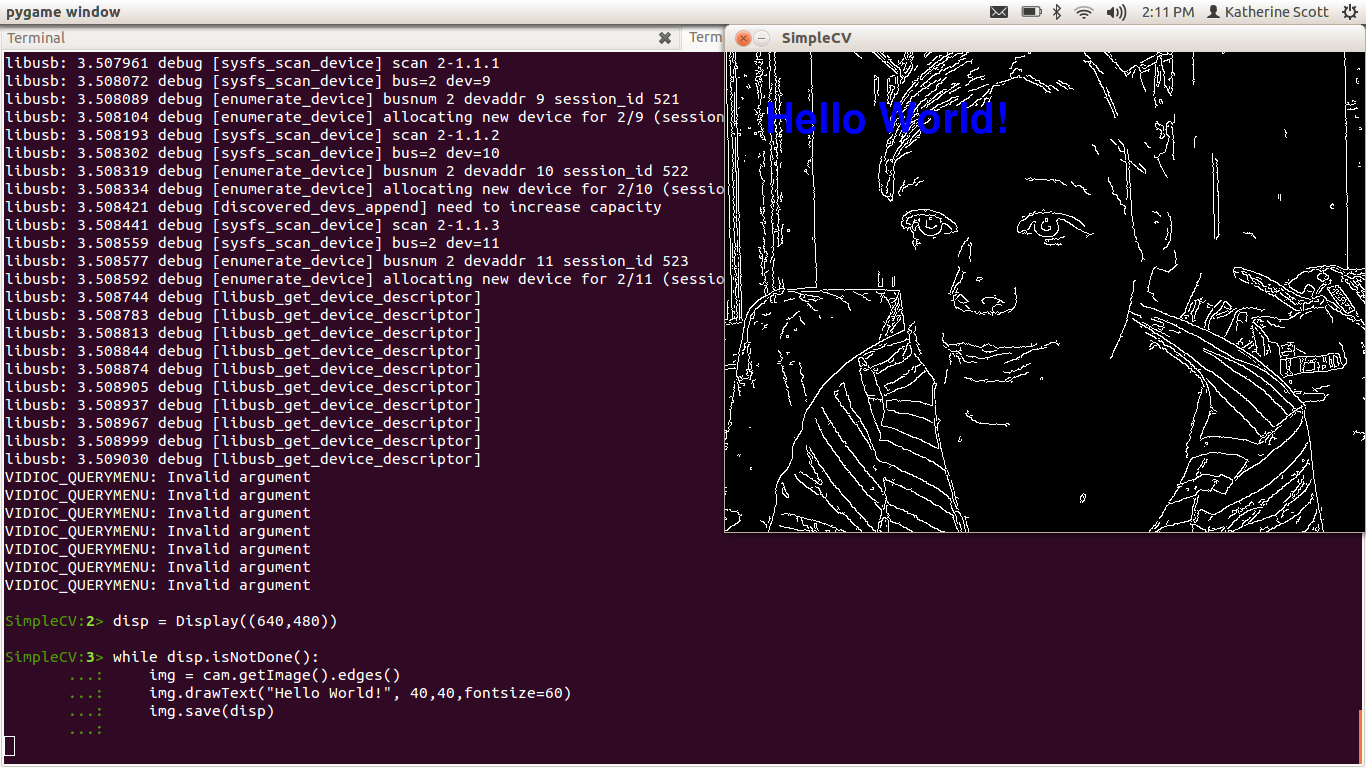
\includegraphics[width=0.9\linewidth]{HelloWorld2.png}
\end{figure}
\end{frame}
% ------------------------------------------------
\subsection{iPython Web Notebook}
% ------------------------------------------------
% ------------------------------------------------
\begin{frame}
\frametitle{Why use iPython Web Notebooks}
\begin{figure}
  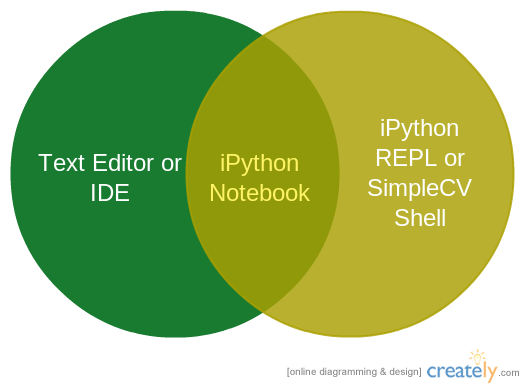
\includegraphics[width=0.7\linewidth]{venn.png}
\end{figure}
\begin{itemize}
\item Web notebooks give you the best features of an IDE and a REPL.
\item You can edit chunks of code, and then execute them in series.
\item iPython is still v. 0.1.4 but it is getting good fast.
\end{itemize}
\end{frame}
% ------------------------------------------------
\begin{frame}
\frametitle{How do I use the notebook?}
\begin{figure}
  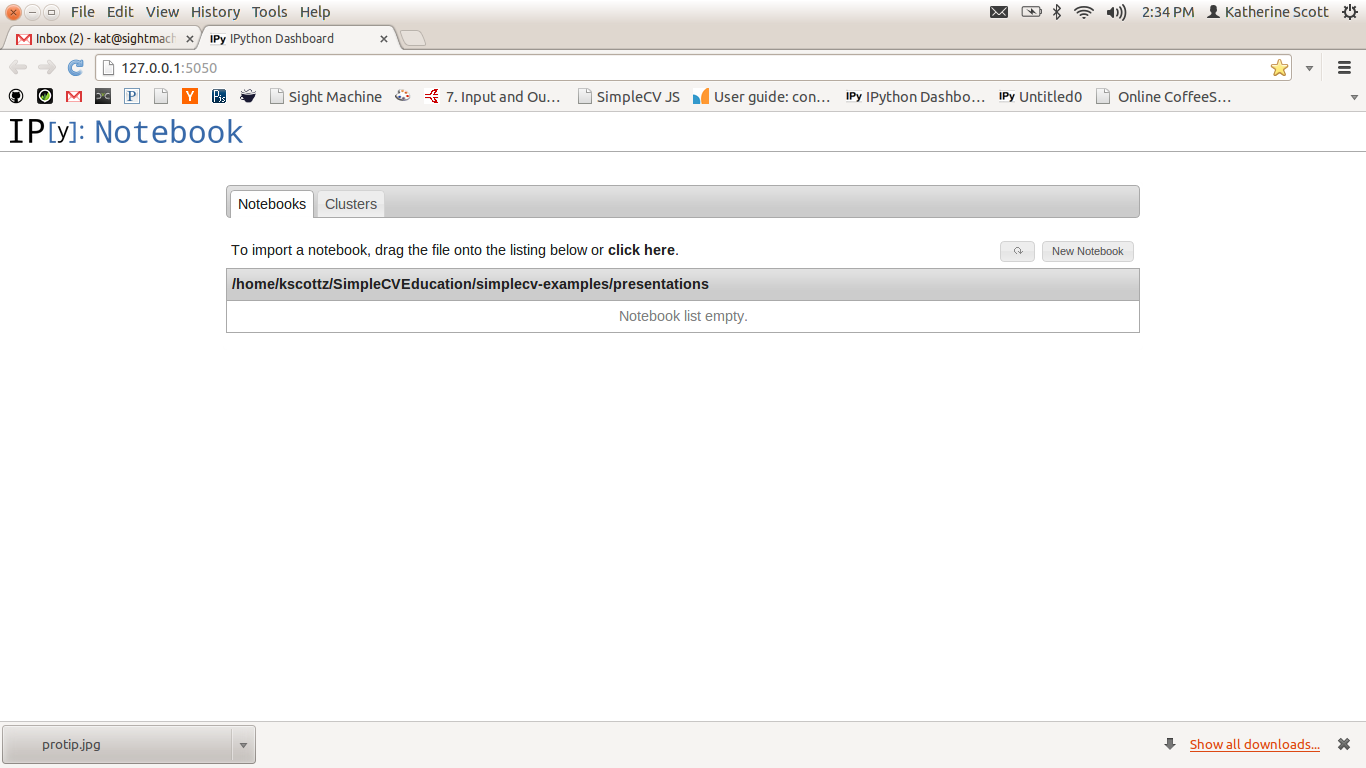
\includegraphics[width=0.5\linewidth]{startingipython.png}
\end{figure}
\begin{itemize}
\item From the shell just type $simplecv$ $notebook$ $--pylab$
  $inline$.
\item The --pylab inline is optional but it pulls in matplotlib which
  is handy.
\item You will get to a dashboard to create a new notebook.
\item By default notebooks are in the path where you start ipython.
\end{itemize}
\end{frame}
% ------------------------------------------------
\begin{frame}
\frametitle{How do I use the notebook?}
\begin{figure}
  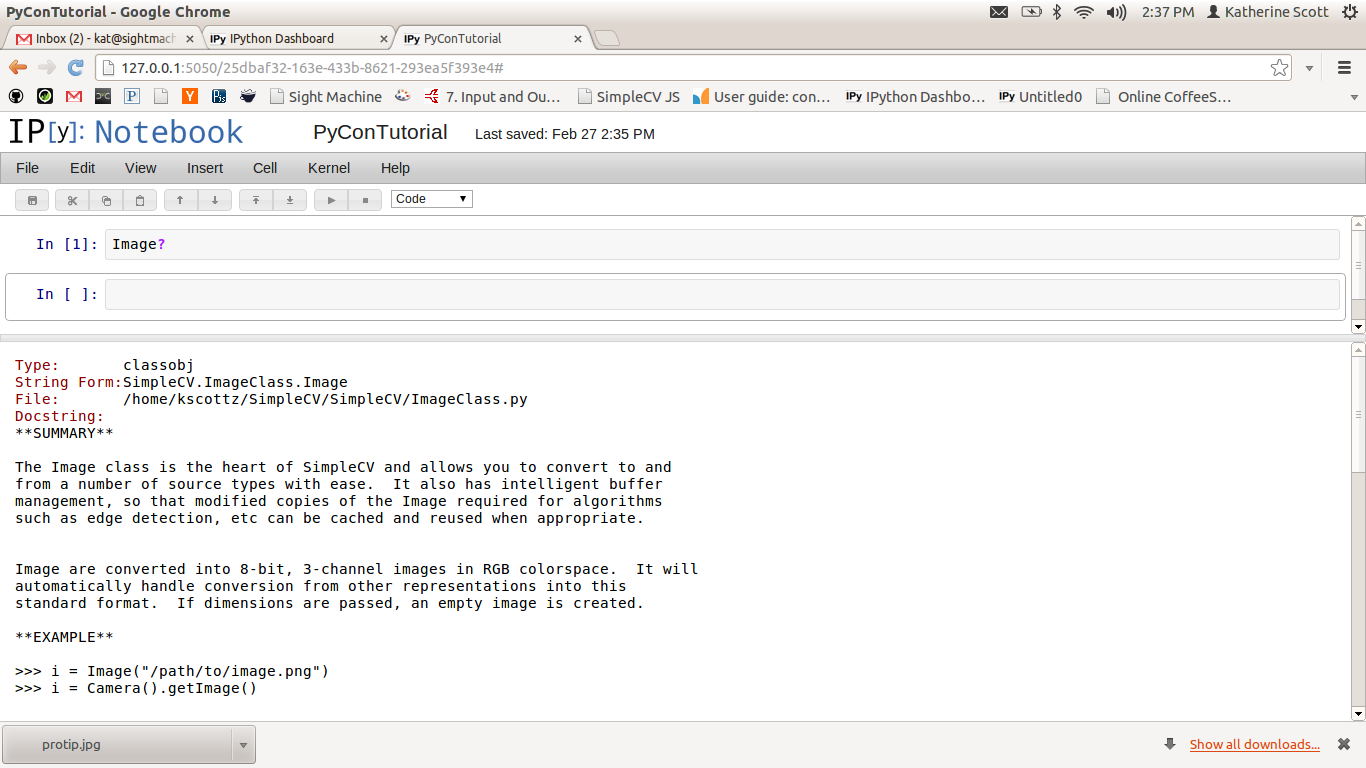
\includegraphics[width=0.7\linewidth]{ipythonHelp.png}
\end{figure}
\begin{itemize}
\item Everything we mentioned about the SimpleCV shell still holds.
\item Magic commands, inline documentation, etc. still work.
\item $enter$ starts a new line.
\item $ctrl-enter$ executes a line.
\end{itemize}
\end{frame}
% ------------------------------------------------
\begin{frame}
\frametitle{Caveats about  iPython Web Notebooks}
\begin{figure}
  
\includegraphics[width=0.2\linewidth]{warning.jpg}
\end{figure}
\begin{itemize}
\item iPython Web Notebooks are still version 0.1.4 
\item \textbf{There is no auto-save. Get in the $ctrl-s$ save habit.}
\item If you edit a module you import you must restart the core. 
\item Minimal editing support. No find/replace.
\item The core can sometimes crash on large images.
\item The notebooks hold on to data by default. This can fill up your
  version control system fast. Try the download as python command from
  the gui. 
\end{itemize}
\end{frame}
% ------------------------------------------------
% ------------------------------------------------
% ------------------------------------------------
 \section{Image Basics}
% % ------------------------------------------------
% % ------------------------------------------------
% % ------------------------------------------------
\begin{frame}
\frametitle{Image Loading Basics II}
\begin{itemize}
\item You can get the image file name using $img.filename$
\item Images can also come from appropriately shaped numpy arrays.
\item PIL and OpenCV images can also be passed into the image.
\item Can also take a URL to an image. 
\item The \alert<+>{img.getEXIFData()} command can show jpg EXIF data.
\end{itemize}
\end{frame}

% % ------------------------------------------------
\begin{frame}
\frametitle{Saving an Image}
\begin{itemize}
\item The \alert<+>{img.save()} command is used to save images.
\item You can save as just about any format, PNG, JPG, WebP, etc.
\item Calling save with no parameters saves it to temp directory.
\item Using the params flag you can set compression, e.g. set
  compression quality. 
\end{itemize}
\end{frame}

% % %------------------------------------------------
\begin{frame}
\frametitle{Using a USB Camera}
\begin{itemize}
\item Most usb cameras use the \alert<+>{Camera} class. 
\item The camera class takes a camera index, \emph{usually} this is the
   order cameras are plugged into the computer.
\item The camera also has properties that you can get and set, or use a propmap dictionary to set. 
 \item \emph{Support for camera properties is vendor specific and spotty at
   best.} 
 \item Cameras also have a \emph{threaded} parameter. Set this to false
 to run multiple cameras. 
\end{itemize}
\end{frame}
% ------------------------------------------------
\frametitle{Using a USB Camera II}
\begin{frame}
\begin{itemize}
\item \alert<+>{Camera.getImage()} will return the current image. 
\item \alert<+>{Camera.getAllProperties()} will return the cameras properties.
\item \alert<+>{Camera.getProperty() and Camera.setProperty()} may let
  you set properties. \emph{This is highly vendor dependent and usually poorly documented.}
\end{itemize}
\end{frame}
%------------------------------------------------
\begin{frame}
\frametitle{Briefly: Other Cameras}
\begin{itemize}
\item Kinect - Depth Camera
\begin{itemize}
\item Uses freenect drivers, not the OpneNI drivers.
\item \alert<+>{Kinect.getImage and Kinect.getDepth }
\item Note that these aren't well calibrated together.
\end{itemize}
\item JpegStreamReader - IP Cameras
\begin{itemize}
\item Give it a url to camera's web feed, and scrape images.
\item Getting the URL straight can be tricky. 
\end{itemize}
\item Virtual Camera
\begin{itemize}
\item A virtual camera that pulls from a directory full of images, or video.
\item Interface to video files for processing.
\end{itemize}
\end{itemize}
\end{frame}
% ------------------------------------------------
\begin{frame}
\frametitle{Briefly: Other Cameras}
\begin{itemize}
\item Document Scanners
\begin{itemize}
\item SANE compatible devices.
\item Allow you to set resolution and ROI. 
\end{itemize}
\item Digital Camera
\begin{itemize}
\item Uses Piggy Photo Library
\item Works with most DSLRs and point and shoots.
\end{itemize}
\item AVT Camera
\begin{itemize}
\item Professional digital imaging cameras with interchangeable optics.
\item Fine grain control of camera parameters. 
\end{itemize}
\end{itemize}
\end{frame}
% ------------------------------------------------
\begin{frame}
\frametitle{Image Sets}
ImageSets are lists of images. They are great for aggregating datasets.
\begin{itemize}
\item By default load all image files in a directory.
\item Can iterate over the list using list comps or for loops.
\item Using the BeautifulSoup library can download sets from google.
\item Can save image sets to directories, or animated gifs!
\item The show command works just like on image class.
\item Can apply averages to images.
\item More coming soon.
\end{itemize}
\end{frame}

% ------------------------------------------------
\begin{frame}[fragile] 
\frametitle{ImageSet Example}
\begin{example}[Image Sets]
\begin{minted}[]{python}
mySet = ImageSet()
mySet.download('cats') # download cats
mySet.show() # show them to us
avgCat = mySet.average() # get the avg cat
avgCat.show() # show the avg cat
mySet[3].show() # show the third kitty
resized = mySet.standardize(128,64)
resized.save('cat.gif')
mySet.save('cat.gif') # save the cats as a gif
for cat in mySet: # iterate over the set of cats
    cat.binarize().show()
\end{minted}
\end{example}
\end{frame}
% ------------------------------------------------
\section{Really Basic Operations}
\subsection{Getting at the Pixels}
\begin{frame}
\frametitle{Getting at a pixel}
\begin{figure}
  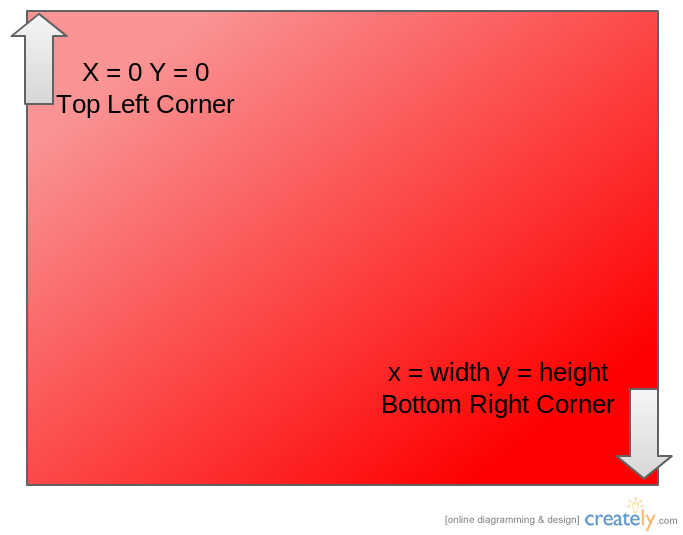
\includegraphics[width=0.5\linewidth]{pixellocations.png}
\end{figure}
\begin{itemize}
\item SimpleCV treats images as two dimensional arrays of color
value tuples. 
\item Each tuple holds three values (Red,Green,Blue).
\item Pixels start in the top left corner at zero. 
\end{itemize}
\end{frame}

% ------------------------------------------------
\begin{frame}[fragile] 
\frametitle{Pixel Manipulation Example}
\begin{example}[Getting at those pixels]
\begin{minted}[fontsize=\tiny]{python}
img = Image('helloworld.jpg')
c = img[0,0] # get a pixel
print c
print img.getPixel(0,0) # get another way
test = img[200:300,200:300]
test.show() # the result is an image
test = img[50:,:]
test.show() # again using slice
test = img[0:5,0:5]
print test.getNumpy() # get the raw values
img[0:105,0:105] = Color.RED 
img.show() # Another way
test = img.getNumpy() #RIGHT!
test[0:105,0:105] = Color.RED
img2 = Image(test)
img2.show()
\end{minted}
\end{example}
\end{frame}
% ------------------------------------------------
\begin{frame}
\frametitle{Getting at a pixel}
\begin{itemize}
\item Images are read only. To write a pixel directly you need create a new
  image. Usually this happens in numpy
\item Images support the list slice notation but return images.
\item To get at the raw pixel values use \textbf{getNumpy()} and \textbf{getGrayNumpy()} 
\item Numpy values can be accessed using slices the first parameter is
  x, the second is y,  and the third is the channel in RGB order. For
  example $npimg[x][y][0]$. 
\item The \textbf{Image.width} and \textbf{Image.height} member
  variables can help you find your way. 
\end{itemize}
\end{frame}
% ------------------------------------------------
\begin{frame}[fragile] 
\frametitle{Another Pixel Manipulation Example}
\begin{example}[Fancy Manipulations]
\begin{minted}[fontsize=\tiny]{python}
img = Image('helloworld.jpg')
gray = img.getGrayNumpy() # get the gray scale np image
colored = img.getNumpy()  # and the colored one
print (img.width,img.height) #tell us the image size
colored[0:20,:] = Color.BLUE # set the left side to blue
colored[:,0:20] = Color.GREEN # set the top row to green
colored[40:80,40:80]      \quad
     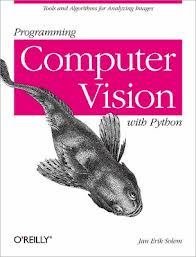
\includegraphics[width=0.4\linewidth]{JanEricBook.jpg}
= Color.YELLOW # make a yellow square
x,y = np.where(gray>230) # find bright pixels > 230
for xf,yf in zip(x,y): # for each of those
    colored[xf][yf] = Color.RED #make them red
img2 = Image(colored) # create an image
img2.show() # and show it
# now set the whole blue channel to 255
colored[:,:,2] = 255 
# and show us that
img3 = Image(colored)
img3.show()
\end{minted}
\end{example}
\end{frame}
% ------------------------------------------------
\begin{frame}
\frametitle{Getting at a pixel}
 \begin{figure}
     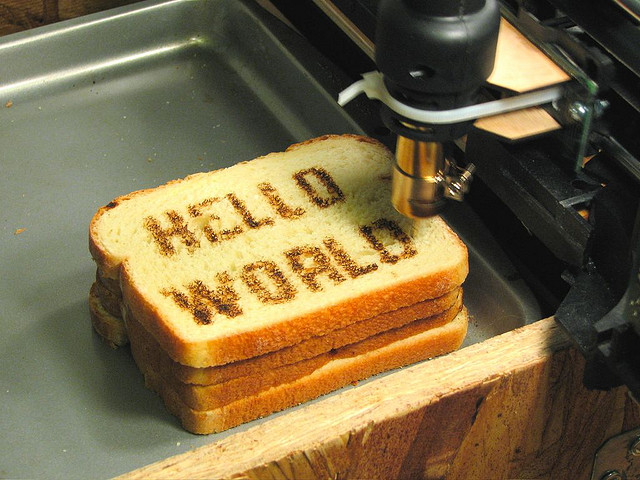
\includegraphics[width=0.3\linewidth]{helloworld.jpg}
     \quad
     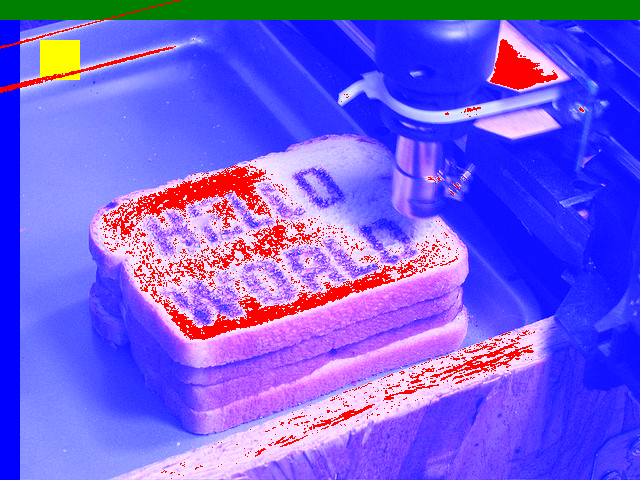
\includegraphics[width=0.3\linewidth]{ColorToast.png}
     \quad
     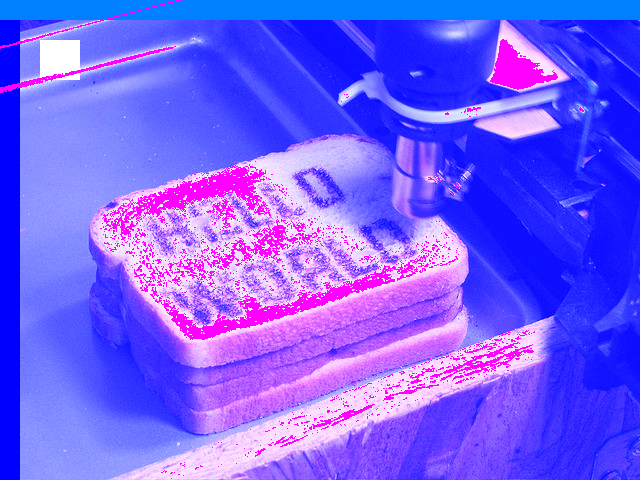
\includegraphics[width=0.3\linewidth]{ColorToast2.png}
     \caption{Not bad for less than 20 lines of code.}
 \end{figure}

\end{frame}
% ------------------------------------------------
\section{Basic Manipulations}
% ------------------------------------------------
\begin{frame}
\frametitle{Cropping, Scaling, Rotating, etc}
It is helpful to think of some image processing like using an image
editor, like GIMP, paint, or that other one Adobe makes. Here are a
few basic image operations you can do in SimpleCV. 
\begin{itemize}
\item \textbf{Image.crop}. Does what it says on the tin. We refer to
  crop areas by there top left corner x and y plus the width height.
\item \textbf{Image.scale} scales the image proportionally while
  \textbf{Image.resize} resizes the image to the desired size. 
  \begin{itemize}
    \item \textbf{Image.resize} is smart, if you tell it a width or
      height it will infer the other parameter from the aspect ratio.
    \item \textbf{Image.scale} uses a proportionality. So passing it
      value of two will double the image size. Make sure to check out
      the interpolation method.
  \end{itemize}
\end{itemize}
\end{frame}
% ------------------------------------------------
\begin{frame}
\frametitle{Rotating}
\begin{itemize}
  \item \textbf{Image.rotate} takes and angle in degrees.
  \item Rotate has a parameter called fixed. If fixed
        is set to false, SimpleCV will create a new image that matches
        the rotated image size. Otherwise we stick the rotated image
        in data in a similarly sized canvas. 
  \item It is possible to pick the x,y position of the rotation. The
    default is the center of the image.
  \item You can also scale an image while rotating.
  \item In a pinch you can use \textbf{Image.flipHorizontal} and
    \textbf{Image.flipVertical}.
   \item Be aware \textbf{FLIPPING != ROTATION}
\end{itemize}
\end{frame}
% ------------------------------------------------
\begin{frame}
\frametitle{Blit}
The \textbf{Image.blit} function gets its name from the old computer graphics term ``bit block image
transfer''. Really it means just copy and paste another image onto
another image and return the result.
\begin{itemize}
\item Blit takes in another image and a position where you want to put
  it.
\item That position can be negative with respect to the destination
  image. For example (-10,-10) would put the source image over the top
  left of the destination image.
\item You can toss blit a binary mask, an alpha value (that is
  transparency) or a an alpha mask (a grayscale image that has an
  alpha mask per pixel).
\end{itemize}
\end{frame}
% ------------------------------------------------
\begin{frame}[fragile] 
\frametitle{Let's play!}
\begin{example}[Basic Manipulations]
\begin{minted}[fontsize=\tiny]{python}
img = Image('tricky.jpg')
face = img.crop(150,190,309-150,333-190)
img.show() # show the source
face.show() # show the cropped image
face.rotate(45).show() # basic rotation
face.rotate(45,fixed=False).show()
face.scale(0.5).show()
face.scale(width=int(face.width/2.0)) # basic scaling
face.flipHorizontal().show() # flipping
test1 = img.blit(face.flipHorizontal(),pos=(150,190))
test1.show() # now let's have fun with blitting
test2 = img.blit(face.flipHorizontal(),pos=(150,190),alpha=0.5)
test2.show() 
mask = Image((face.width,face.height))
# Here we are just drawing a white circle on a black background
mask.drawCircle((face.width/2,face.height/2),70,color=Color.WHITE, thickness=-1)
mask = mask.applyLayers()
mask.show()
test3 = img.blit(face.flipHorizontal(),pos=(150,190),mask=mask)
test3.show()
face.binarize().blur().show()
test4 = img.blit(face.flipHorizontal(),pos=(150,190),alphaMask=face.binarize().blur())
test4.show()
\end{minted}
\end{example}
\end{frame}
% ------------------------------------------------
\begin{frame}
\frametitle{The Blit Progression of President Dick Nixon}
 \begin{figure}
     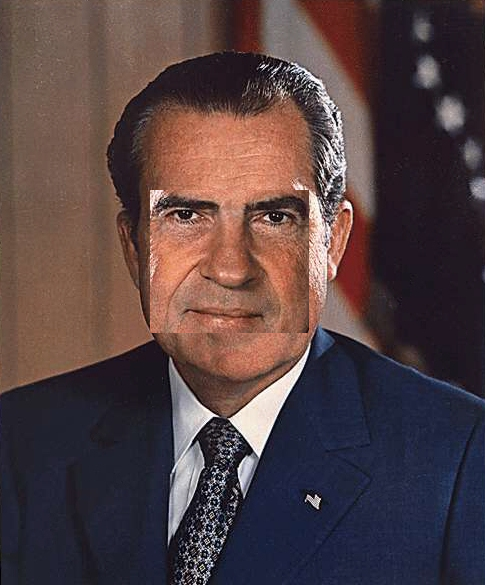
\includegraphics[width=0.2\linewidth]{tricky1.png}
     \quad
     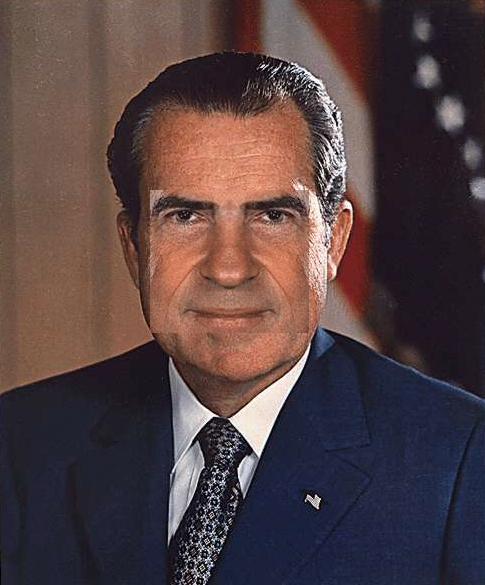
\includegraphics[width=0.2\linewidth]{tricky2.png}
     \quad
     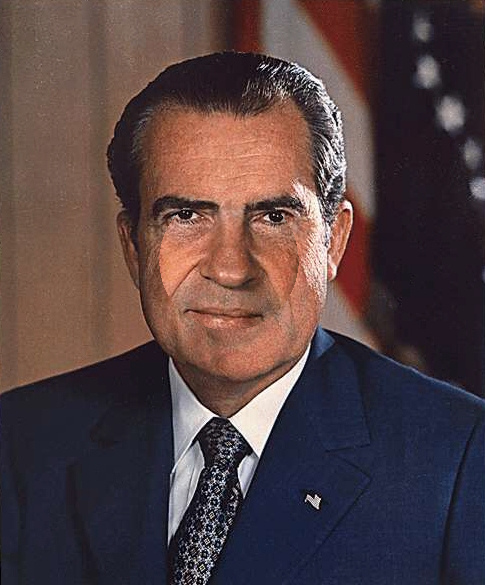
\includegraphics[width=0.2\linewidth]{tricky3.png}
     \quad
     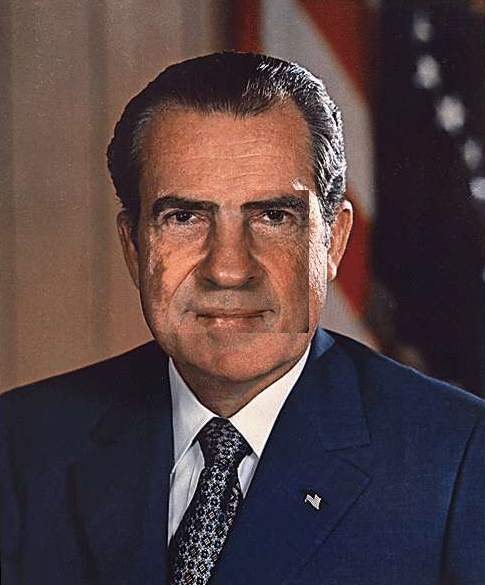
\includegraphics[width=0.2\linewidth]{tricky4.png}
     \quad
     \caption{Various blitting}
 \end{figure}
\large{Can you our subject a smaller face or a slightly slanted face? }
\end{frame}
% ------------------------------------------------
\begin{frame}
\frametitle{A few more basics}
\begin{itemize}
  \item \textbf{Image.blur} - A basic Gaussian blur. 
  \item \textbf{Image.smooth} - A variety of smoothing filters. Some
    good for removing camera noise. 
  \item \textbf{Image.toGray} - Convert a color image to a gray scale
    image.
  \item \textbf{Image.threshold} - Take an image and set all off the
    pixels that have a grayscale value above the threshold to white,
    and everything else to black.
 \item \textbf{Image.invert} - Swap the lightest and darkest values,
   like a photo negative. 
\end{itemize}
\end{frame}
% ------------------------------------------------

\section{Let's talk about black, white, and color}
% ------------------------------------------------
\begin{frame}
\frametitle{Let's Talk about color, color spaces, and much more.}
 \begin{figure}
     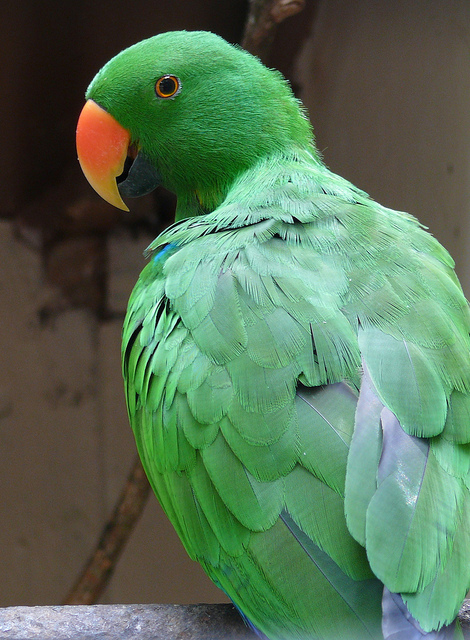
\includegraphics[width=0.2\linewidth]{parrot.jpg}
     \quad
     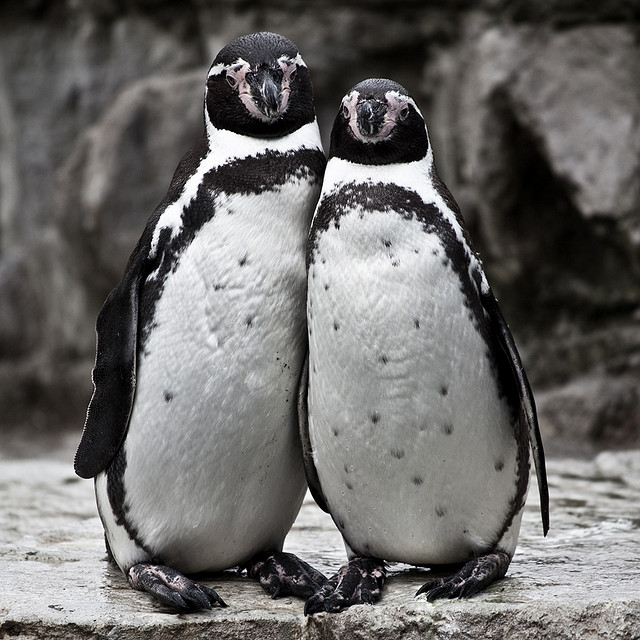
\includegraphics[width=0.3\linewidth]{penguins.jpg}
 \end{figure}
Computer vision is all about moving from a vast amount of
information to small result as quickly as possible. Working in
grayscale, or black and white images can speed things up
dramatically. 
\end{frame}

% ------------------------------------------------
\begin{frame}
\frametitle{Color is surprisingly hard to represent}
 \begin{figure}
     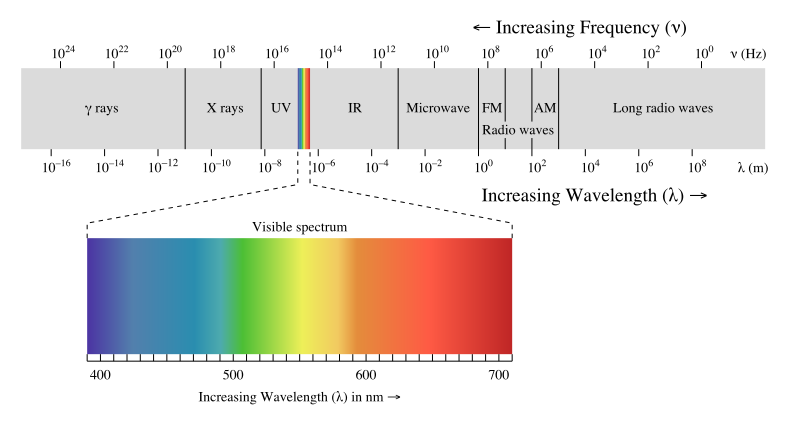
\includegraphics[width=0.3\linewidth]{visiblelight.png}
     \quad
     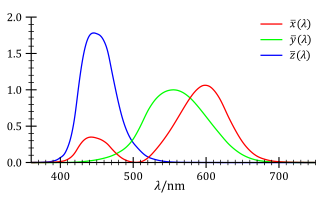
\includegraphics[width=0.3\linewidth]{theeye.png}
     \quad
     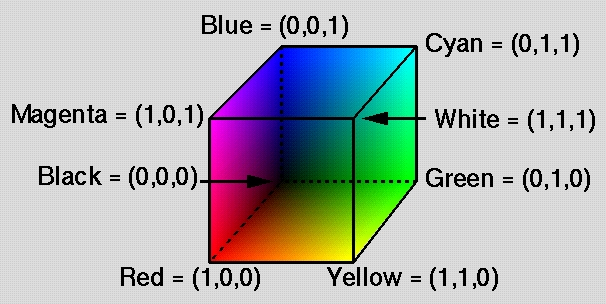
\includegraphics[width=0.3\linewidth]{RGB_cube_color.jpg}
 \end{figure}
We start with visible light, which bounces around, does funky stuff, and then enters our
eye or camera. Our eyes and cameras have a response function that does
an imperfect job of sampling the parts of the spectrum. We then take
those samples and try to map them onto finite color space like RGB. 
\end{frame}

% ------------------------------------------------
\begin{frame}
\frametitle{An illustration of why color is hard.}
 \begin{figure}
     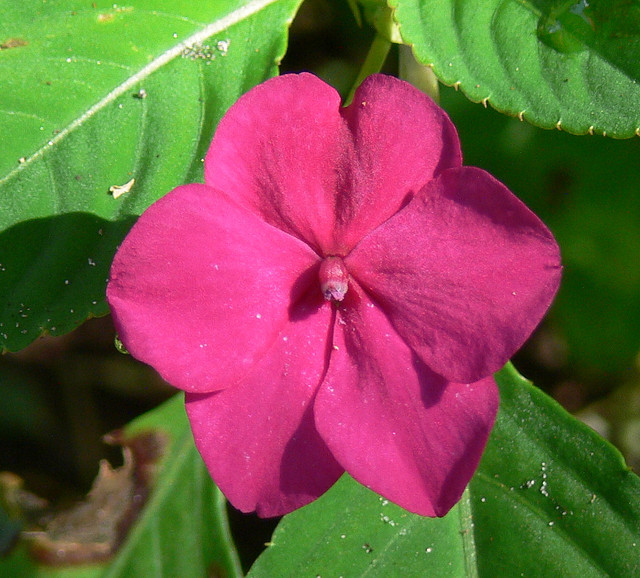
\includegraphics[width=0.3\linewidth]{flower.jpg}%
     \quad
     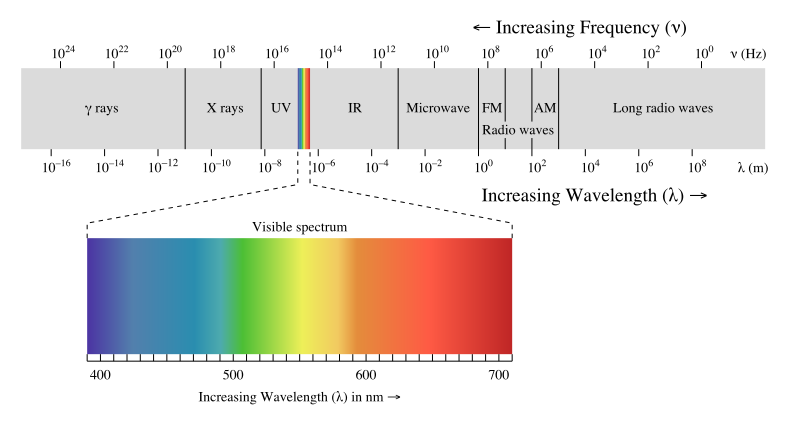
\includegraphics[width=0.5\linewidth]{visiblelight.png}%
 \end{figure}
Point to where this magenta flower lives on the visible light spectrum.
\end{frame}
% ------------------------------------------------
\begin{frame}
\frametitle{MIND BLOWN!}
 \begin{figure}
     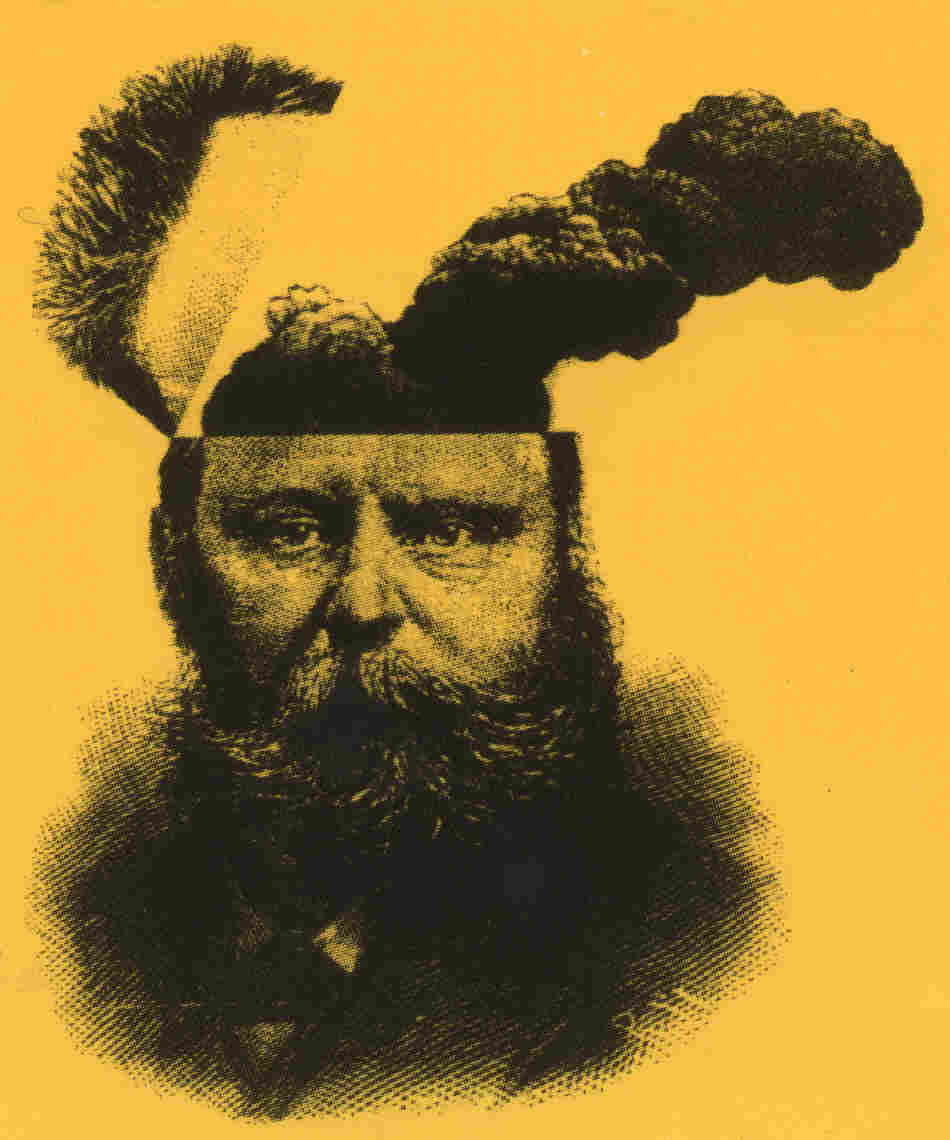
\includegraphics[width=0.3\linewidth]{mindblown.jpg}
 \end{figure}
Magenta doesn't exist in nature. It is trick our brains and cameras
play on us. It exists because we sample the spectrum and try to
recombine the samples. We wrap the visible spectrum around. 
\end{frame}
% ------------------------------------------------
\begin{frame}
\frametitle{To manage this problem we use color spaces.}
 \begin{figure}
     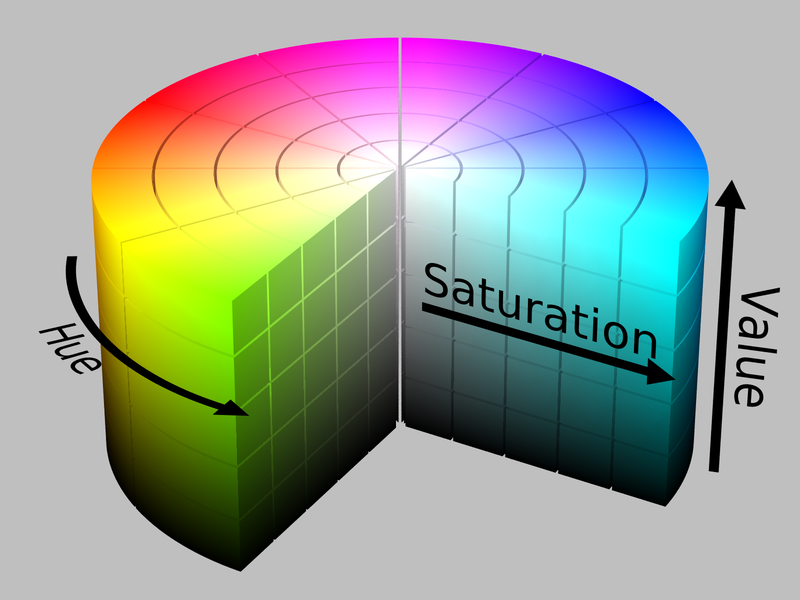
\includegraphics[width=0.4\linewidth]{hsv.png}
 \end{figure}
\begin{itemize}
\item To deal with this problem we use color spaces. 
\item Most images are in the RGB, BGR, or gray scale color spaces.
\item Sometimes it is helpful to use the hue, saturation, and value (HSV)
color space. In HSV you have a 
\begin{itemize}
\item Hue, or pure color (from 0 to 180) 
\item Saturation that tells us how far from white our color is
\item Value that tells us how dark the color is.
\end{itemize}
\end{itemize}
\end{frame}


% ------------------------------------------------
\begin{frame}
\frametitle{How do I work with Color in SimpleCV}
\begin{itemize}
\item The \textbf{Image.toHSV()} function will convert your image, while the
\textbf{Image.toBGR()} function will return it back to the original.
\item We also have \textbf{Image.toGray()} and \textbf{Image.toRGB()}
  and whole bunch more. 
\item The \textbf{Image.huePeaks} function can help you guess what
  hues are in your image.
\item The \textbf{Image.hueDistance} function can then help you look
  for stuff that is the hue you want. 
\item The \textbf{Image.hueHistogram} function will let you visualize
  the results. 
\end{itemize}
\end{frame}
\begin{frame}[fragile] 
% ------------------------------------------------
\frametitle{Finding colors}
\begin{example}[Using Hue]
\begin{minted}[fontsize=\tiny]{python}
import pylab as plt # import pylab for plotting
img = Image("flower.jpg")
img.show()
peaks = img.huePeaks() # find the hues
print peaks
hist = img.hueHistogram() # get the histogram too
plt.plot(hist) # plot the histogram
plt.draw() # show it to us
# show how far away from the hue we are black is closer
# white is farther away from our hue.
hdist = img.hueDistance(peaks[3][0]) 
# create a black and white version of our flower
binary = img.hueDistance(peaks[3][0]).invert().threshold(220)
hdist.show()
binary.show()
hdist.save('hflower.png')
binary.save('bflower.png')
\end{minted}
\end{example}
\end{frame}
% ------------------------------------------------
\begin{frame}
\frametitle{Color Finding Results}
 \begin{figure}
     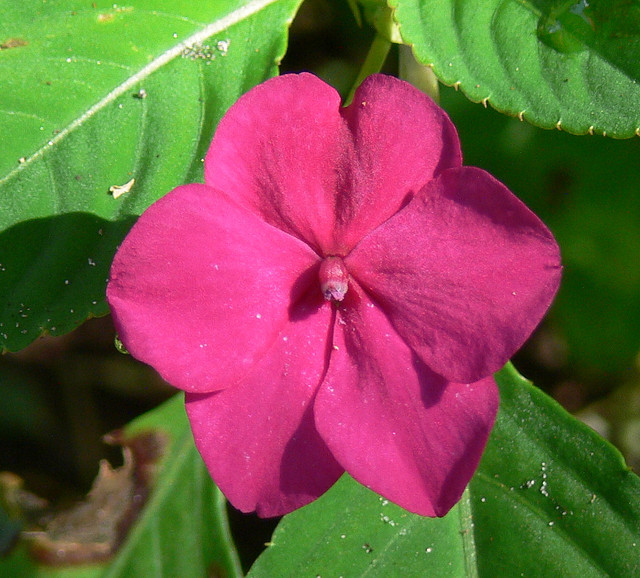
\includegraphics[width=0.3\linewidth]{flower.jpg}
     \quad
     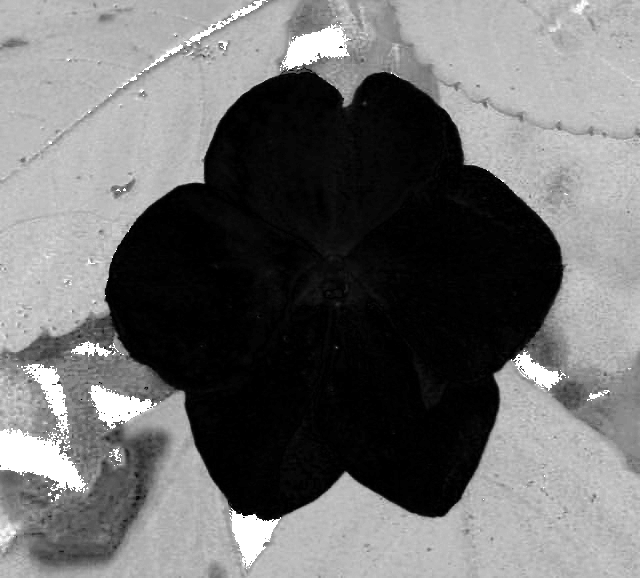
\includegraphics[width=0.3\linewidth]{hflower.png}
     \quad
     
\includegraphics[width=0.3\linewidth]{bflower.png}
     \quad
     \caption{Finding an object from colors}
 \end{figure}
\end{frame}


\begin{frame}
  \frametitle{Paragraphs of Text}
  Sed iaculis dapibus gravida. Morbi sed tortor erat, nec interdum arcu. Sed id lorem lectus. Quisque viverra augue id sem ornare non aliquam nibh tristique. Aenean in ligula nisl. Nulla sed tellus ipsum. Donec vestibulum ligula non lorem vulputate fermentum accumsan neque mollis.\\~\\

  Sed diam enim, sagittis nec condimentum sit amet, ullamcorper sit
  amet libero. Aliquam vel dui orci, a porta odio. Nullam id suscipit
  ipsum. Aenean lobortis commodo seDerkt commodo leo gravida
  vitae. Pellentesque vehicula ante iaculis arcu pretium rutrum eget
  sit amet purus. Integer ornare nulla quis neque ultrices
  lobortis. Vestibulum ultrices tincidunt libero, quis commodo erat
  ullamcorper id.
\end{frame}

% ------------------------------------------------

\begin{frame}
  \frametitle{Bullet Points}
  \begin{itemize}
  \item Lorem ipsum dolor sit amet, consectetur adipiscing elit
  \item Aliquam blandit faucibus nisi, sit amet dapibus enim tempus eu
  \item Nulla commodo, erat quis gravida posuere, elit lacus lobortis
    est, quis porttitor odio mauris at libero
  \item Nam cursus est eget velit posuere pellentesque
  \item Vestibulum faucibus velit a augue condimentum quis convallis
    nulla gravida
  \end{itemize}
\end{frame}

% ------------------------------------------------

\begin{frame}
  \frametitle{Multiple Columns}

  \begin{columns}[c] % The "c" option specifies centered vertical alignment while the "t" option is used for top vertical alignment

    \column{.45\textwidth} % Left column and width
    \textbf{Heading}
    \begin{enumerate}
    \item Statement
    \item Explanation
    \item Example
    \end{enumerate}

    \column{.5\textwidth} % Right column and width
    Lorem ipsum dolor sit amet, consectetur adipiscing elit. Integer
    lectus nisl, ultricies in feugiat rutrum, porttitor sit amet
    augue. Aliquam ut tortor mauris. Sed volutpat ante purus, quis
    accumsan dolor.

  \end{columns}
\end{frame}


\begin{frame}
\frametitle{Table}
\begin{table}
\begin{tabular}{l l l}
\toprule
\textbf{Treatments} & \textbf{Response 1} & \textbf{Response 2}\\
\midrule
Treatment 1 & 0.0003262 & 0.562 \\
Treatment 2 & 0.0015681 & 0.910 \\
Treatment 3 & 0.0009271 & 0.296 \\
\bottomrule
\end{tabular}
\caption{Table caption}
\end{table}
\end{frame}

%------------------------------------------------

\begin{frame}
\frametitle{Theorem}
\begin{theorem}[Mass--energy equivalence]
$E = mc^2$
\end{theorem}
\end{frame}

%------------------------------------------------


\begin{frame}[fragile] % Need to use the fragile option when verbatim is used in the slide
\frametitle{Verbatim}
\begin{example}[Theorem Slide Code]
\begin{minted}{python}

  def doStuff(a,b,c=[1,2,3]):
      a = 5
      b = a 
      c.reverse()
  
  derp = [1,2,3,4]
  for i in derp:
     doStuff()
     pass
  print deep

\end{minted}
\end{example}
\end{frame}


\begin{frame}[fragile] % Need to use the fragile option when verbatim is used in the slide
\frametitle{Verbatim}
\begin{example}[Theorem Slide Code]
\begin{verbatim}

$E = mc^2$

\end{verbatim}
\end{example}
\end{frame}

%------------------------------------------------

\begin{frame}
\frametitle{Figure}
Uncomment the code on this slide to include your own image from the same directory as the template .TeX file.
%\begin{figure}
%\includegraphics[width=0.8\linewidth]{test}
%\end{figure}
\end{frame}

%------------------------------------------------

\begin{frame}[fragile] % Need to use the fragile option when verbatim is used in the slide
\frametitle{Citation}
An example of the \verb|\cite| command to cite within the presentation:\\~

This statement requires citation \cite{p1}.
\end{frame}

%------------------------------------------------

\begin{frame}
\frametitle{References}
\footnotesize{
\begin{thebibliography}{99} % Beamer does not support BibTeX so references must be inserted manually as below
\bibitem[Smith, 2012]{p1} John Smith (2012)
\newblock Title of the publication
\newblock \emph{Journal Name} 12(3), 45 -- 678.
\end{thebibliography}
}
\end{frame}

%------------------------------------------------

\begin{frame}
\Huge{\centerline{The End}}
\end{frame}

%----------------------------------------------------------------------------------------

\end{document} 
